%% (Master) Thesis template
% Template version used: v1.4
%
% Largely adapted from Adrian Nievergelt's template for the ADPS
% (lecture notes) project.


%% We use the memoir class because it offers a many easy to use features.
\documentclass[11pt,a4paper,titlepage]{report}

%% Packages
%% ========

%% LaTeX Font encoding -- DO NOT CHANGE
\usepackage[OT1]{fontenc}

%% Babel provides support for languages.  'english' uses British
%% English hyphenation and text snippets like "Figure" and
%% "Theorem". Use the option 'ngerman' if your document is in German.
%% Use 'american' for American English.  Note that if you change this,
%% the next LaTeX run may show spurious errors.  Simply run it again.
%% If they persist, remove the .aux file and try again.
\usepackage[english]{babel}

%% Input encoding 'utf8'. In some cases you might need 'utf8x' for
%% extra symbols. Not all editors, especially on Windows, are UTF-8
%% capable, so you may want to use 'latin1' instead.
\usepackage[utf8]{inputenc}

%% This changes default fonts for both text and math mode to use Herman Zapfs
%% excellent Palatino font. Do not change this.
\usepackage[sc]{mathpazo}

%% The AMS-LaTeX extensions for mathematical typesetting.  Do not
%% remove.
\usepackage{amsmath,amssymb,amsfonts,mathrsfs}

%% NTheorem is a reimplementation of the AMS Theorem package. This
%% will allow us to typeset theorems like examples, proofs and
%% similar.  Do not remove.
%% NOTE: Must be loaded AFTER amsmath, or the \qed placement will
%% break
\usepackage[amsmath,thmmarks]{ntheorem}

%% LaTeX' own graphics handling
\usepackage{graphicx}

%% We unfortunately need this for the Rules chapter.  Remove it
%% afterwards; or at least NEVER use its underlining features.
\usepackage{soul}

%% This allows you to add .pdf files. It is used to add the
%% declaration of originality.
\usepackage{pdfpages}
\usepackage{blindtext}

%% Make document internal hyperlinks wherever possible. (TOC, references)
%% This MUST be loaded after varioref, which is loaded in 'extrapackages'
%% above.  We just load it last to be safe.
\usepackage[linkcolor=black,colorlinks=true,citecolor=black,filecolor=black]{hyperref}


%% Document information
%% ====================

\title{Classification and Detection of Untrimmed Videos Using Recurrent Neural Networks}
\author{Alberto Montes}
% \thesistype{Master Thesis}
% \advisors{Advisors: Prof.\ Dr.\ A. D. Visor, Dr.\ P. Ostdoc}
% \department{Department of Computer Science}
\date{June 26, 2016}

\begin{document}

%% Title page is autogenerated from document information above.  DO
%% NOT CHANGE.
\begin{titlepage}
    \maketitle
\end{titlepage}

%% The abstract of your thesis.  Edit the file as needed.
\chapter*{Acknowledgements}
\pagenumbering{arabic}
First of all I would like to thank my two tutors of this project, Xavier Giró-i-Nieto and Amaia
Salvador for guiding and teaching me during all this project.

\chapter*{Abstract}

This thesis explore different approaches using Convolutional and Recurrent Neural Networks to classify and temporally localize activities on videos, furthermore an implementation to achieve it has been proposed.

As the first step, features have been extracted from video frames using an state of the art 3D Convolutional Neural Network. This features are fed in a recurrent neural network that solves the activity classification and temporally location tasks in a simple and flexible way.

Different architectures and configurations have been tested in order to achieve the best performance and learning of the video dataset provided. In addition it has been studied different kind of post processing over the trained network's output to achieve a better results on the temporally localization of activities on the videos.

The results provided by the neural network developed in this thesis have been submitted to the ActivityNet Challenge 2016 of the CVPR, achieving competitive results using a simple and flexible architecture.

\chapter*{Resumen}

Esta tesis explora diferentes enfoques usando Redes Neuronales Convolucionales y Redes Neuronales Recurrentes para clasificar y localizar temporalmente actividades en videos y propone una implementación propia.

Como primer paso, se han extraido descriptores de videos usando Redes Neuronales Convolucionales 3D del estado del arte. Estos descriptores se introducen en una Red Neuronal Recurrente que resuelve la clasificación de actvidades y su localización temporal de una manera simple y flexible.

Diferentes arquitecturas y configuraciones se han testeado con el objetivo de conseguir el mejor resultado y aprendizaje del conjunto de vídeos subministrado. Además, se han estudiado diferentes tipos de post procesado sobre la salida de la red entrenada para conseguir mejores resultados en la localización de actividades en los vídeos.

Los resultados obtenidos por la red neuronal desarrollada en esta tesis han sido publicados en la ActivityNet Challenge 2016 del CVPR consiguiendo resultados competitivos con una simple y flexible arquitectura.

\chapter*{Resum}

Aquesta tesis explora diferents enfocaments utilitzant Xarxes Neuronals Convolucionals i Xarxes Neuronals Recurrents per classificar i localitzar temporalment activitats en videos i proposa una implementació pròpia.

Com a primer pas, s'han extret descriptors de videos utilitzant Xarxes Neuronals Convolutionals 3D de l'estat de l'art. Aquests descriptors s'han introduït en una Xarxa Neuronal Recurren que resol la classificació d'activitats i la seva localització temporal d'una manera simple i flexible.

Diferents arquitectures i configuracions han estat testejades amb l'objectiu d'aconseguir el millor resultat i aprenentatge del conjunt de videos subministrats. A més, s'ha estudiat diferents tipus de post processat sobre la sortida de la xarxa entrenada per aconseguir els millors resultats en la localització d'activitats en els videos.

Els resultats obtinguts per la xarxa neuronal desenvolupada en aquesta tesis han estat publicats a la ActivityNet Challenge 2016 del CVPR aconseguint resultats competitius amb una simple i flexible arquitectura.


%% TOC with the proper setup, do not change.
\tableofcontents
\listoffigures
\listoftables

%% Your real content!
\chapter{Introduction}

\section{Statement of Purpose}

Recognizing activities in videos has become a hot topic over the last years in the computer vision community~\cite{ngiam2011multimodal}. The exponential growth of portable video cameras and online multimedia repositories, as well as recent advances in video coding, storage and computational resources have motivated an intense research in the field towards new and more efficient solutions for organizing, understanding and retrieving video content.

Deep learning techniques have recently become the new state of the art in many computer vision tasks, such as image and object recognition in still images. While successful methodologies have been presented for image understanding, video content still presents additional challenges (e.g. motion, temporal consistency, ...)  that often cannot be bridged with still image recognition solutions.  

The purpose of this work is to address the challenges of video content analysis taking advantage of state-of-the-art deep learning techniques. The aim of this project is to develop a competitive framework to both classify and temporally localize activities on videos. To achieve this goal, the dataset used to fulfill this task is be the ActivityNet dataset \cite{caba2015activitynet}, which offers untrimmed videos depicting a diversity of human activities.

%Rather than focusing on activity classification on videos, the aim of this project is to offer a good framework to detect and localize activities on videos. To achieve this goal, the dataset used to fulfill this task will be the ActivityNet dataset \cite{caba2015activitynet}, which offers untrimmed videos which a huge variety of activities on it.

% AMAIA: I think that it is fine to say that you will both address activity classification and detection in your thesis, not just detection... DONE

In particular, this project's main contributions are:
\begin{itemize}
	\item The design and training of a deep learning model architecture, which is based on 3D Convolutional features and Recurrent Neural Networks.
    \item The development and analysis of post processing techniques for classification and temporal localization
    \item The release of an open sourced package containing all the tools to reproduce the experiments, as well as the conversion of a state-of-the-art C3D model from Caffe to Keras.
    
% REMOVED:    \item A framework to classify and localize activities on videos using deep learning techniques, more precisely using recurrent neural networks.
%    \item Develop techniques to process sequence output from Recurrent Neural Networks, to get the activities' localization on videos.
%    \item Explore different configurations of Neural Networks to achieve the best results in activity classification and detection.
%    \item Contribute to the research community porting a model to extract features from video from one deep learning framework to another and open sourcing the code.
\end{itemize}

% AMAIA: I am not sure whether these are your contributions or a summary list of everything you did in the thesis. For contributions, I would stick to:
% 1) The design and training of the architecture, which is based on 3D conv features and RNNs
% 2) The development & analysis of postprocesssing techniques for classification & detection
% 3) The release of an opensourced package containing all the tools to reproduce the experiments, as well as the conversion of a state-of-the-art 3CD model from Caffe to Keras.

This project has been developed at the \textit{Image Processing Group (GPI) of the Universitat Politecnica de Catalunya (UPC)} during the Spring 2016 semester. This group had already work in deep learning techniques for still images, but never before in video analytics. %In this sense, this is a pioneering work that sets a baseline technique and software for future research within the group. 
%REMOVED: This project has no baseline and all the code and development of deep learning techniques applied to video has been done from scratch.
% AMAIA: What do you mean with this sentence? I guess this is assumed in all projects unless stated otherwise... ALBERTO: I tried to say that it has all been done from scratch with no previous work on this field on the Image group.

\section{Requirements and Specifications}

This project has been developed with the implicit goal of seeting a baseline for video analytics with deep learning in the research group, so that future students and researchers to keep working on it. The requirements of this project are the following:
\begin{itemize}
    \item Design and train a deep neural network to classify and temporally localize activities on videos using the ActivityNet Dataset.
    \item Participate in the ActivityNet Challenge 2016, organized as a workshop in the top conference IEEE Conference on Computer Vision and Pattern Recognition (h5-index = 128).
\end{itemize}

% AMAIA: I guess that by requirements you mean "what you were asked to do/what we agreed to do" at the beginning of the project? I slightly modified it, uut feel free to add more items.

As this project has been developed from scratch, no prior specifications were defined. The specifications were decided taking into account the needs for the project and the available resources. All the development was done on \textit{Python} using a very well-known framework which is \textit{Keras}, also a pioneering use of this library in GPI. This Deep Learning wrapper facilitates the design and training of models over two computational frameworks: \textit{Theano}\cite{theano2016theano} and \textit{TensorFlow}\cite{abadi2016tensorflow}. Both  projects support complex and high demanding computations over both CPU and GPU. For this project \textit{Theano} was used as backend because, at the time of developing this project, it was the only one that had implemented the convolution 3D and max pooling 3D operations required for its development.

In addition to the software, specific hardware was required. The high demanding computational resources needed to train neural networks required the use of GPUs provided by the \textit{Image Processing Group} at UPC.

%DELETED: For the development of Deep Learning models and to do all the computations were used some frameworks in \textit{Python}. Because this project has been developed without a baseline, no prior specifications were required. Anyway, for the development of this project it has been decided to work with \textit{Python} for development and \textit{Keras} over \textit{Theano}\cite{theano2016theano} as the deep learning framework to use.

% AMAIA: "Anyway" is too informal...
% AMAIA: I don't know if this applies here, but what about the GPUs that you used? ALBERTO: I've just added

\section{Methods and Procedures}

\textcolor{red}{XAVI: I guess you do not know what to write here, is that right ? \\ALBERTO: Right. \\XAVI: I suggest you always follow as a guideline Andrea Calafell's thesis. Here, she offered a summary of her work. You could do the same, by just copying here part of the Abstract you wrote in the working notes. Check Andrea's thesis here: https://imatge.upc.edu/web/publications/fine-tuning-convolutional-network-cultural-event-recognition}

\section{Work Plan}

This project was planned to follow the packages detailed on this section, with the exception of some minor deviations described in Section~\ref{section:work_plan_deviations}.

\subsection{Work Packages}

\begin{itemize}
    \item WP 1: Project Documentation
    \item WP 2: Research for the State of the Art
    \item WP 3: Dataset to work with
    \item WP 4: Software to use
    \item WP 5: Experimentation and Results Evaluation
    \item WP 6: ActivityNet Challenge 2016 Participation
    \item WP 7: Delivery and Exposition of this project
\end{itemize}

\subsection{Gantt Diagram}

The Gantt diagram of this project's work plan can be found on the Figure~\ref{fig:gantt_diagram}.

\begin{figure}[H]
\begin{center}
% Em falta fer-lo 
%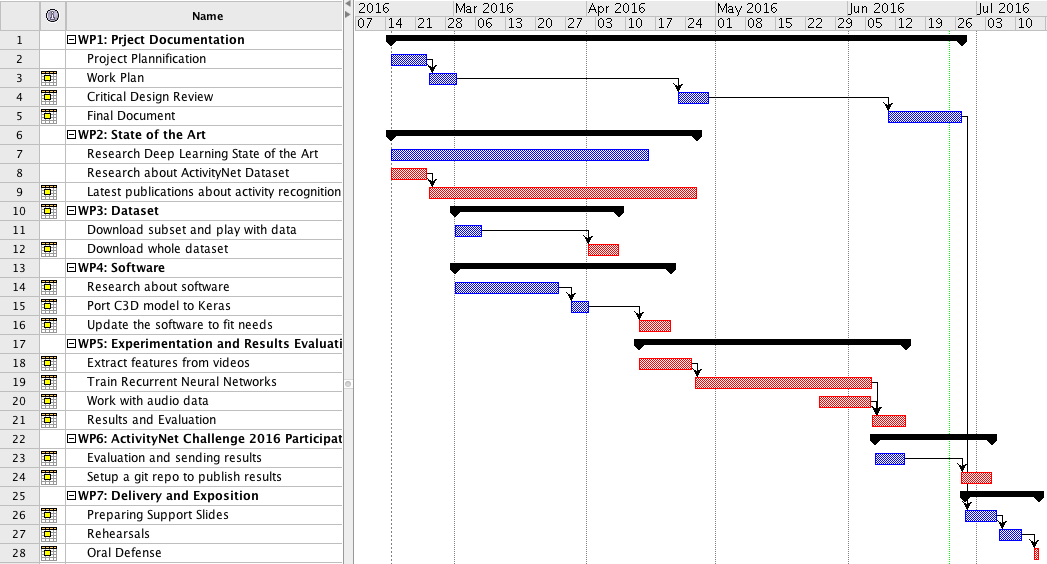
\includegraphics[width=1\linewidth]{img/introduction/gantt_diagram}
\end{center}
\caption{Gantt diagram of this thesis.}
\label{fig:gantt_diagram}
\end{figure}

\textcolor{red}{XAVI: Do not forget your Gannt diagram. You can always check the meetings notes I took if you do not remeber the exact timing of each task. This document should help you in revieweing everything you have been doing since February.}


\section{Work Plan Deviations and Incidents}
\label{section:work_plan_deviations}

The initial plan was to adapt the C3D\cite{tran2014learning} model for the ActivityNet task, which is implemented with the  \textit{Caffe} deep learning framework. But in order to use Recurrent Neural Networks, \textit{Keras} was a much better and flexible framework, so it was necessary to export the original C3D model from the Caffe framework to Keras.

Another deviation for the plan was that, due to the huge amount of required computational resources, fine tuning the full C3D network was not been possible. Instead, the C3D framework was used to extract features from the videos, which were later used as inputs to train the recurrent neural network.

Finally, the original work plan was extended by exploring the potential of audio descriptors for activity recognition. For this task, this work was supported by Professor Ignasi Esquerra from the TALP research group at UPC. He took care of extracting the audio features, which were later assessed and fused with the visual ones.


\appendix

\chapter{Results Figures}

\begin{figure}[H]
\begin{center}
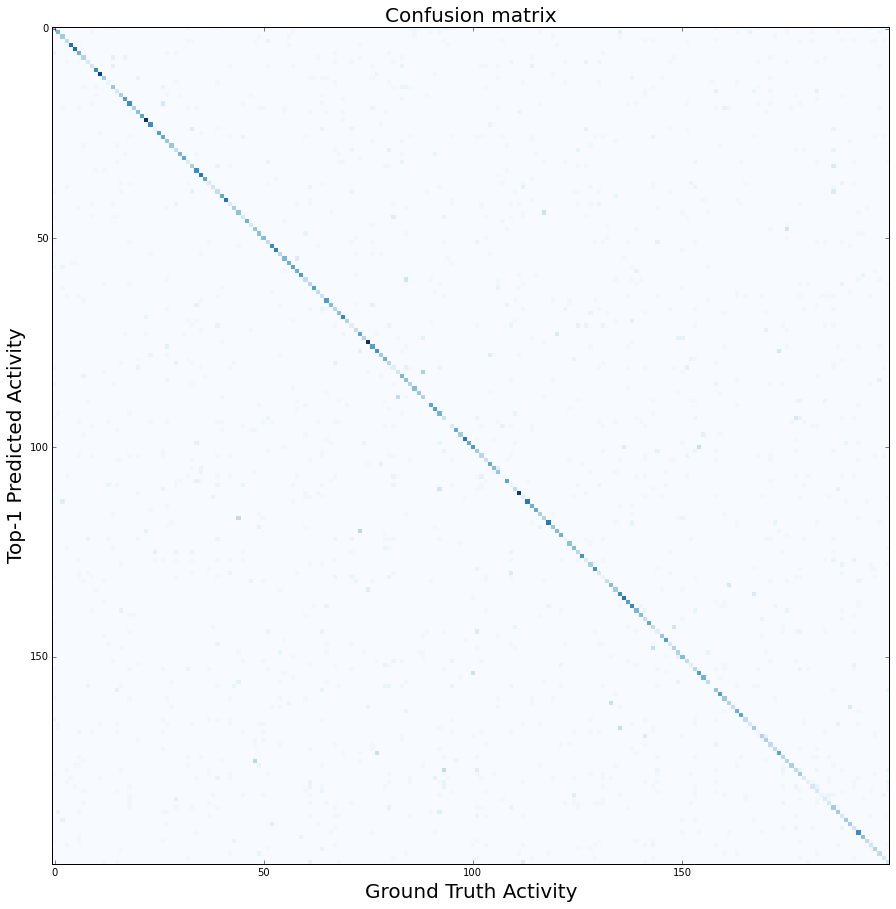
\includegraphics[width=1\linewidth]{img/results/confussion_matrix}
\end{center}
\caption{Confusion matrix of the top-1 activity predicted with the ground truth}
\label{fig:confussion_matrix}
\end{figure}


\begin{figure}[H]
\centering
\begin{subfigure}[b]{.4\textwidth}
  \texttt{Video ID: c-zbA4zixfE \\
  Activity: Throwing darts \\
  \\
  Prediction: \\
  0.7325	Throwing darts \\
  0.1364	Baking cookies \\
  0.0254	Playing blackjack \\}
\end{subfigure}%
\begin{subfigure}[b]{.6\textwidth}
  \centering
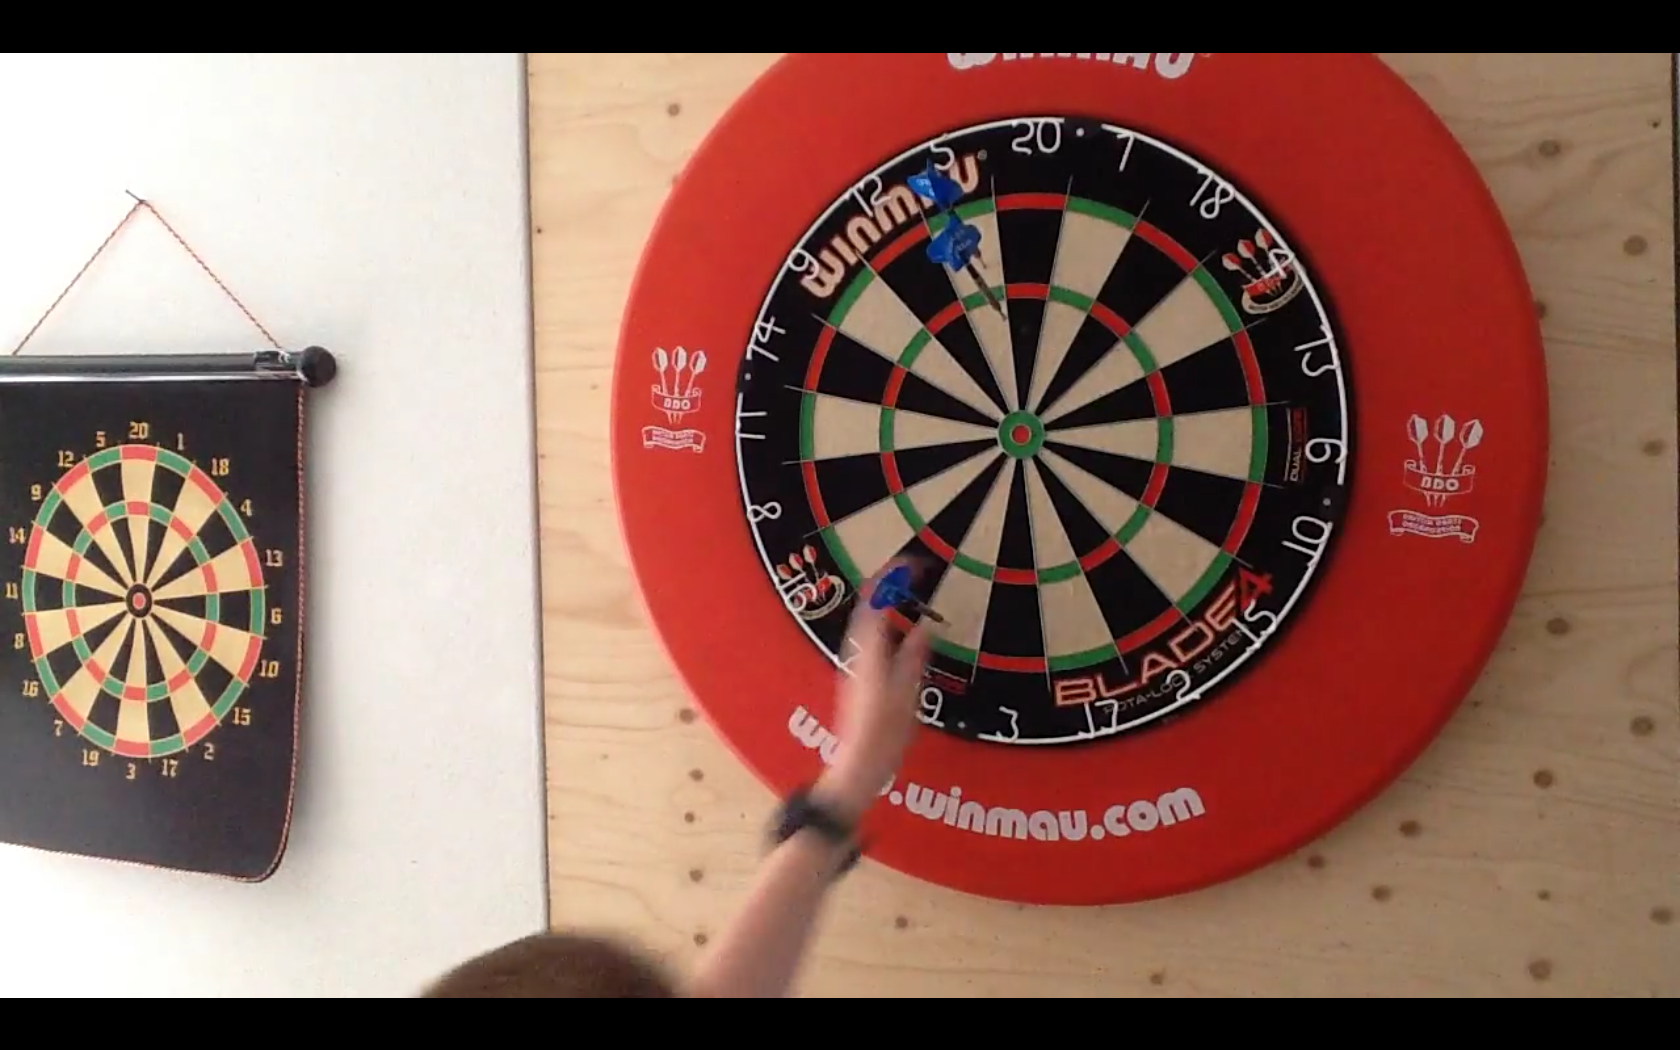
\includegraphics[width=0.95\linewidth]{img/results/activity_classification/results_visualization_classification_5}
\end{subfigure}

\begin{subfigure}[b]{.4\textwidth}
  \texttt{Video ID: p8MvTi8hJdE \\
    Activity: Snowboarding \\
    \\
    Prediction: \\
    0.5043	Skiing \\
    0.2683	Snowboarding \\
    0.1637	Snow tubing \\}
\end{subfigure}%
\begin{subfigure}[b]{.6\textwidth}
  \centering
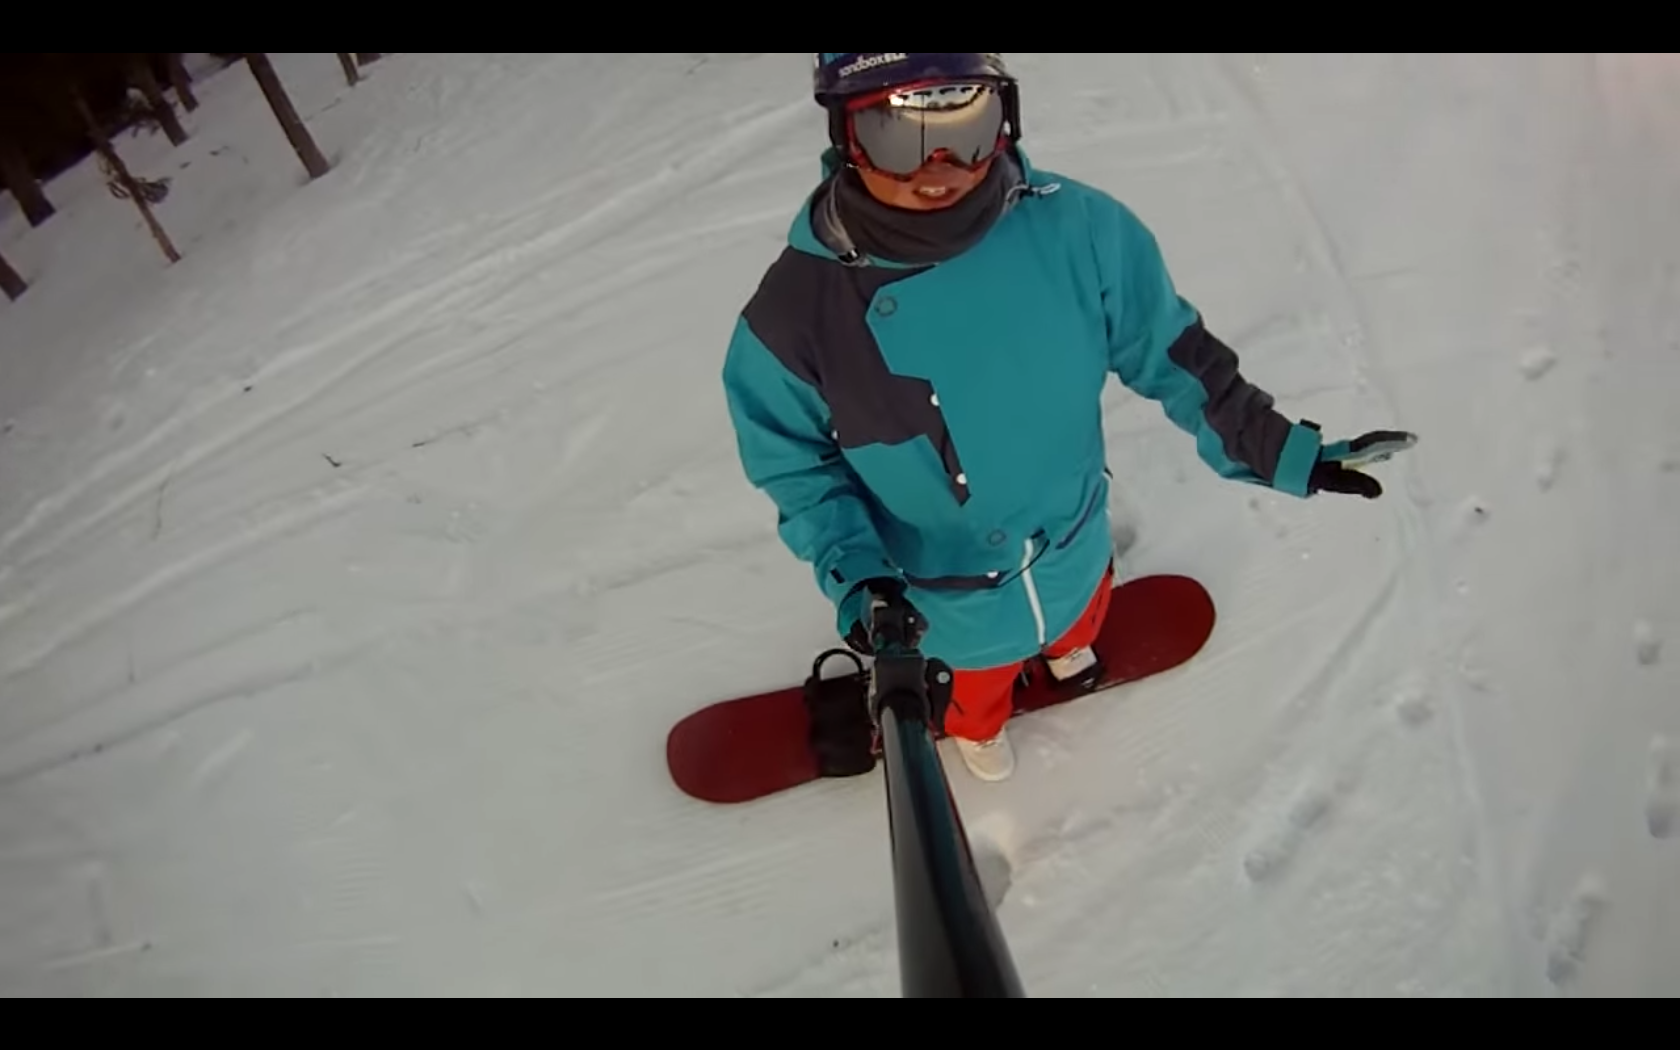
\includegraphics[width=0.95\linewidth]{img/results/activity_classification/results_visualization_classification_6}
\end{subfigure}

\begin{subfigure}[b]{.4\textwidth}
  \texttt{Video ID: ATk8OkvNHHQ \\
    Activity: BMX \\
    \\
    Prediction: \\
    0.9099	BMX \\
    0.0413	Doing motocross \\
    0.0103	Paintball \\}
\end{subfigure}%
\begin{subfigure}[b]{.6\textwidth}
  \centering
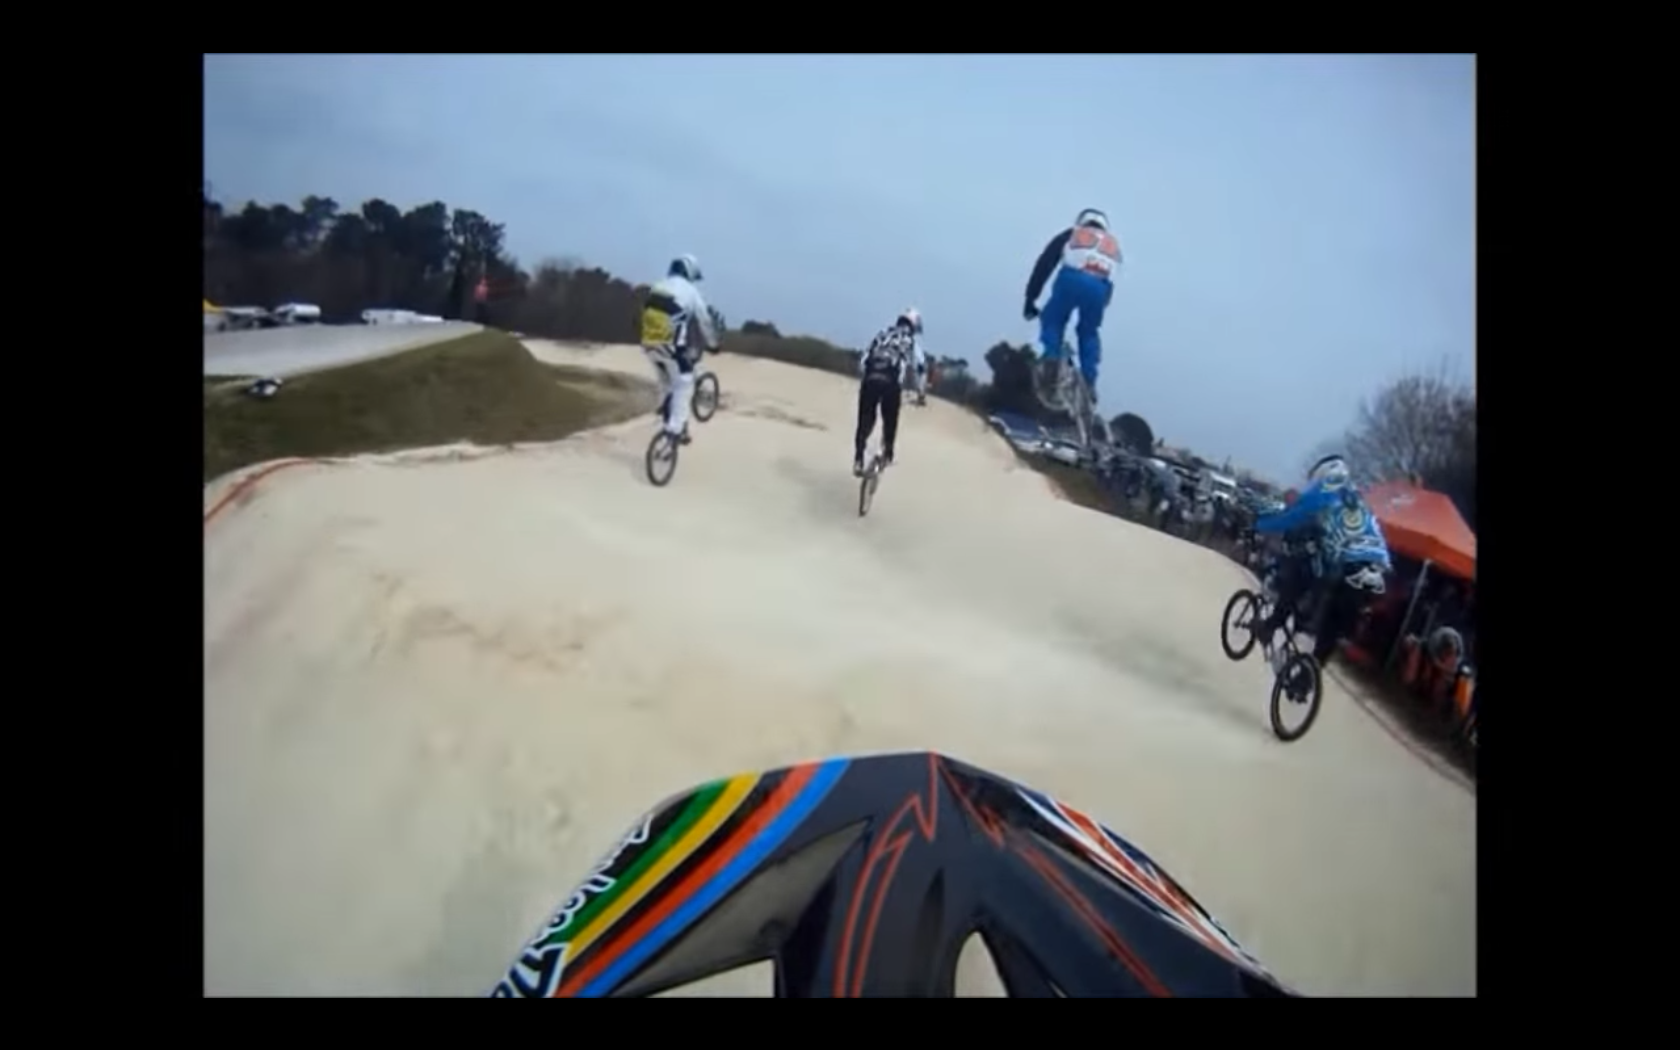
\includegraphics[width=0.95\linewidth]{img/results/activity_classification/results_visualization_classification_7}
\end{subfigure}

\begin{subfigure}[b]{.4\textwidth}
  \texttt{Video ID: -uR5-jYe0Ag \\
  Activity: Putting on makeup \\
  \\
  Prediction: \\
  0.1035	Smoking a cigarette \\
  0.1002	Getting a haircut \\
  0.0941	Putting on makeup \\}
\end{subfigure}%
\begin{subfigure}[b]{.6\textwidth}
  \centering
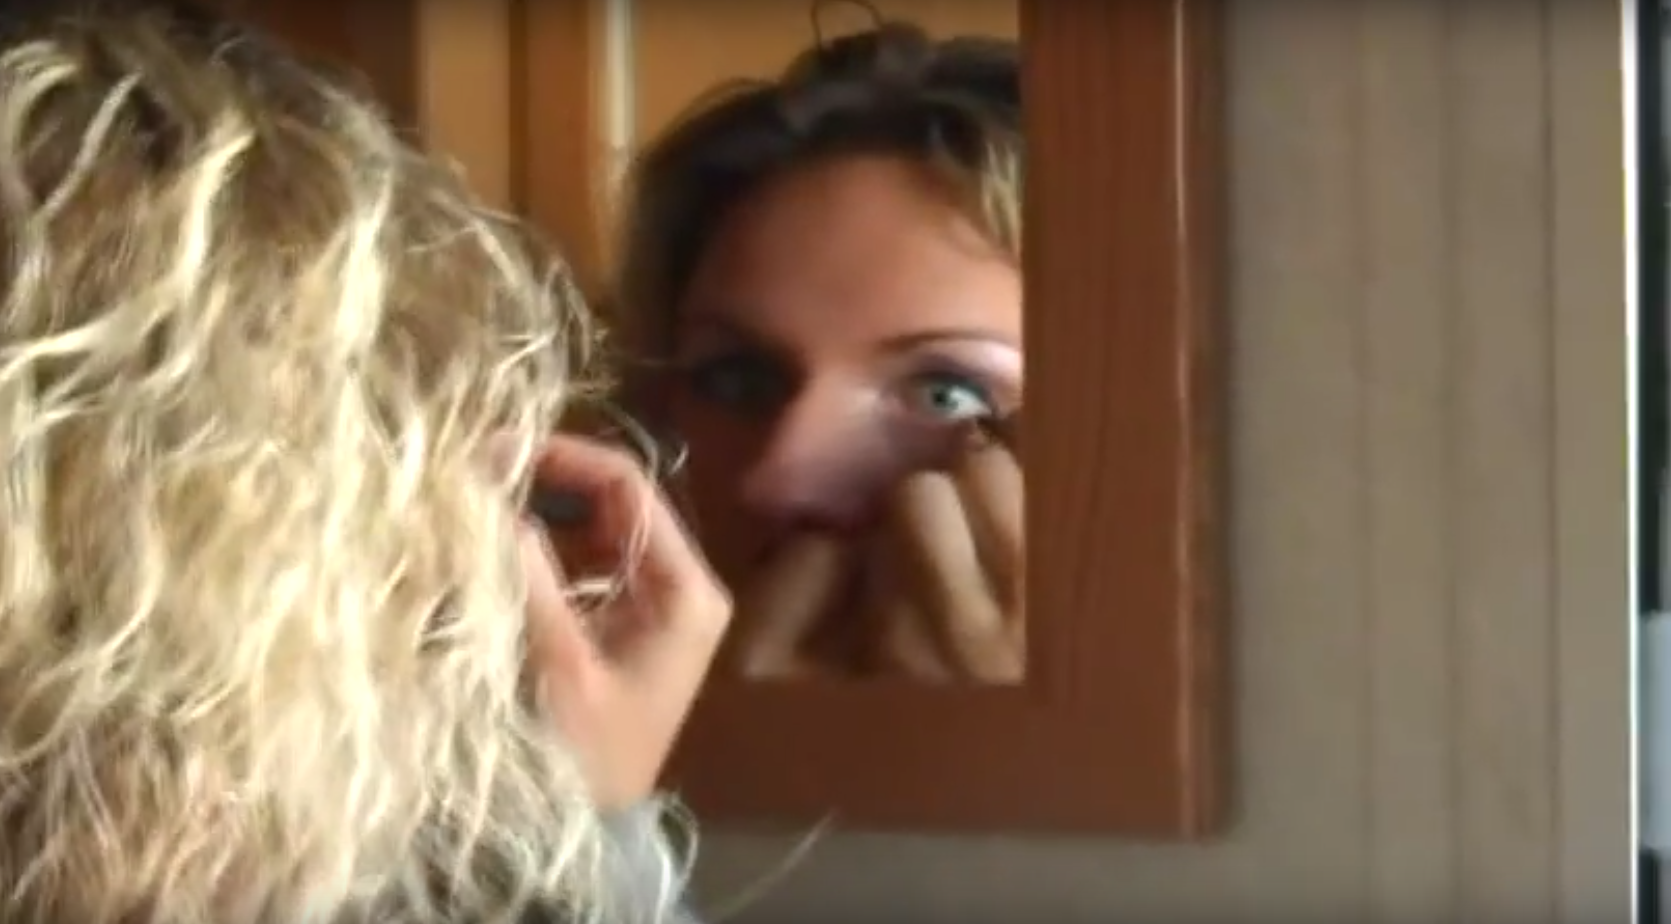
\includegraphics[width=0.95\linewidth]{img/results/activity_classification/results_visualization_classification_8}
\end{subfigure}

\caption{Results for the classification task}
\label{fig:results_visualization_classification_annex_1}
\end{figure}

\begin{figure}[H]
\centering
\begin{subfigure}[b]{.4\textwidth}
  \texttt{Video ID: vc820BteGzY \\
    Activity: Making a cake \\
    \\
    Prediction: \\
    0.3165	Making a lemonade \\
    0.1073	Putting on makeup \\
    0.0768	Making a cake \\}
\end{subfigure}%
\begin{subfigure}[b]{.6\textwidth}
  \centering
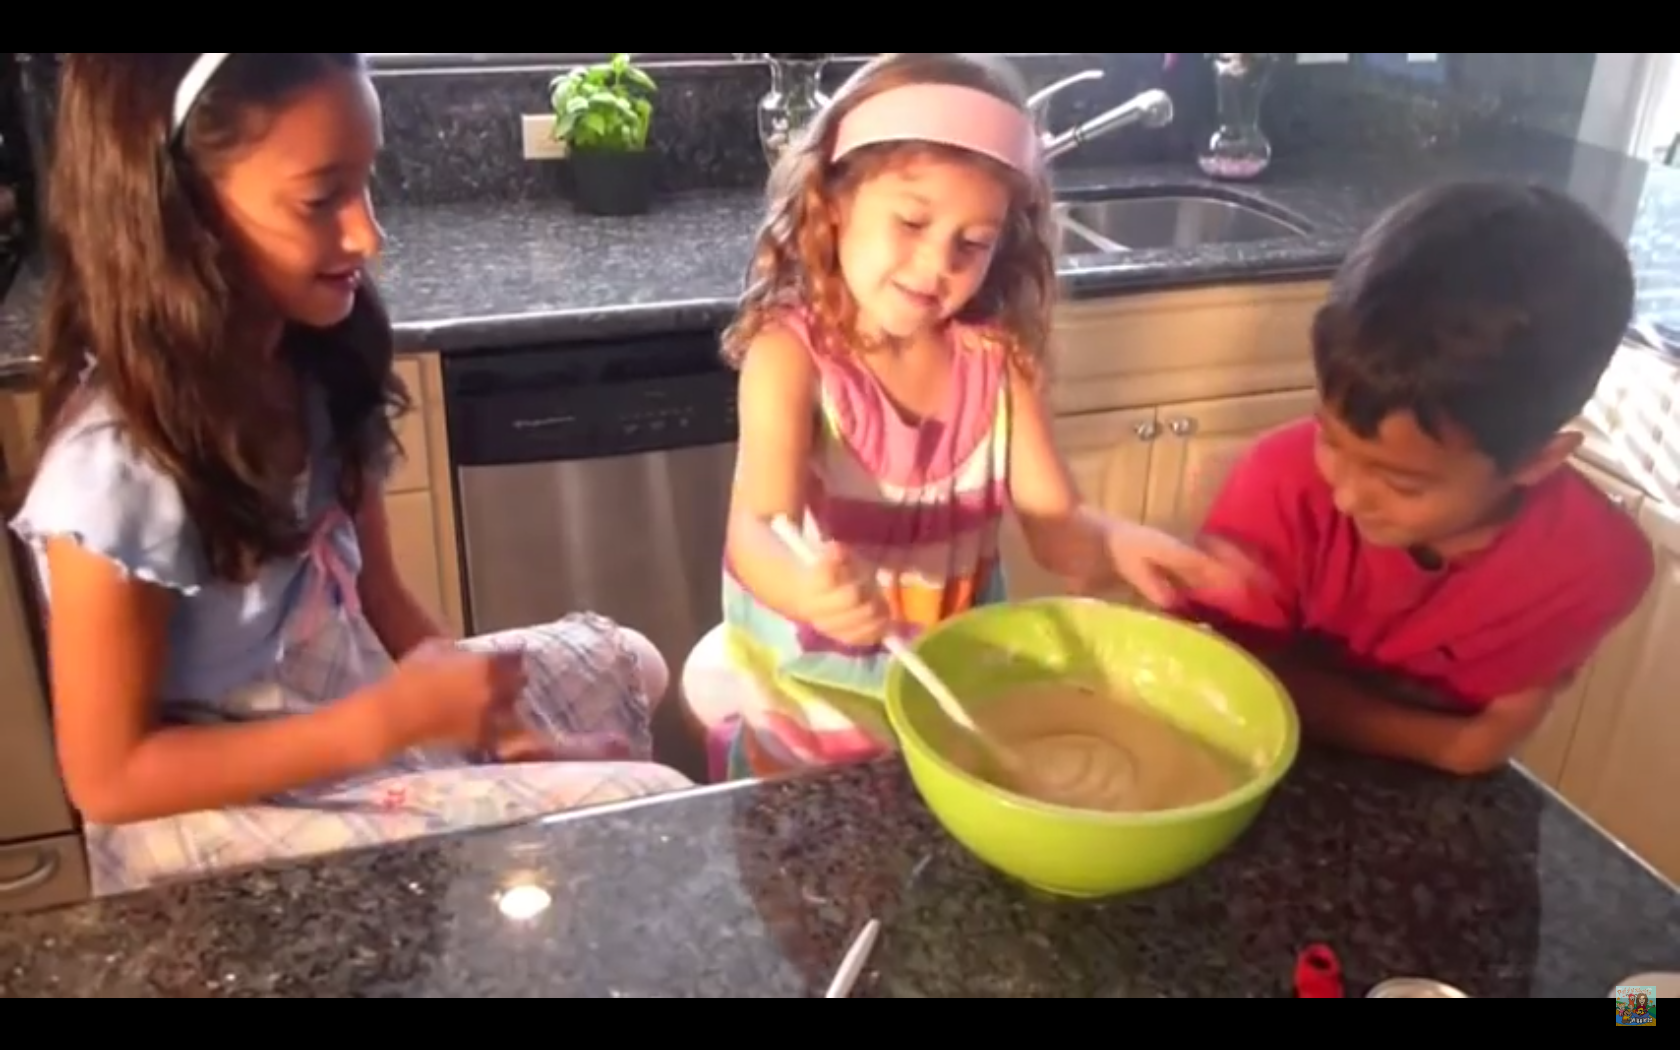
\includegraphics[width=0.95\linewidth]{img/results/activity_classification/results_visualization_classification_9}
\end{subfigure}

\begin{subfigure}[b]{.4\textwidth}
  \texttt{Video ID: tBNOJJx4Z9k \\
    Activity: Hand washing clothes \\
    \\
    Prediction: \\
    0.4742	Cleaning sink \\
    0.0728	Washing hands \\
    0.0497	Baking cookies \\}
\end{subfigure}%
\begin{subfigure}[b]{.6\textwidth}
  \centering
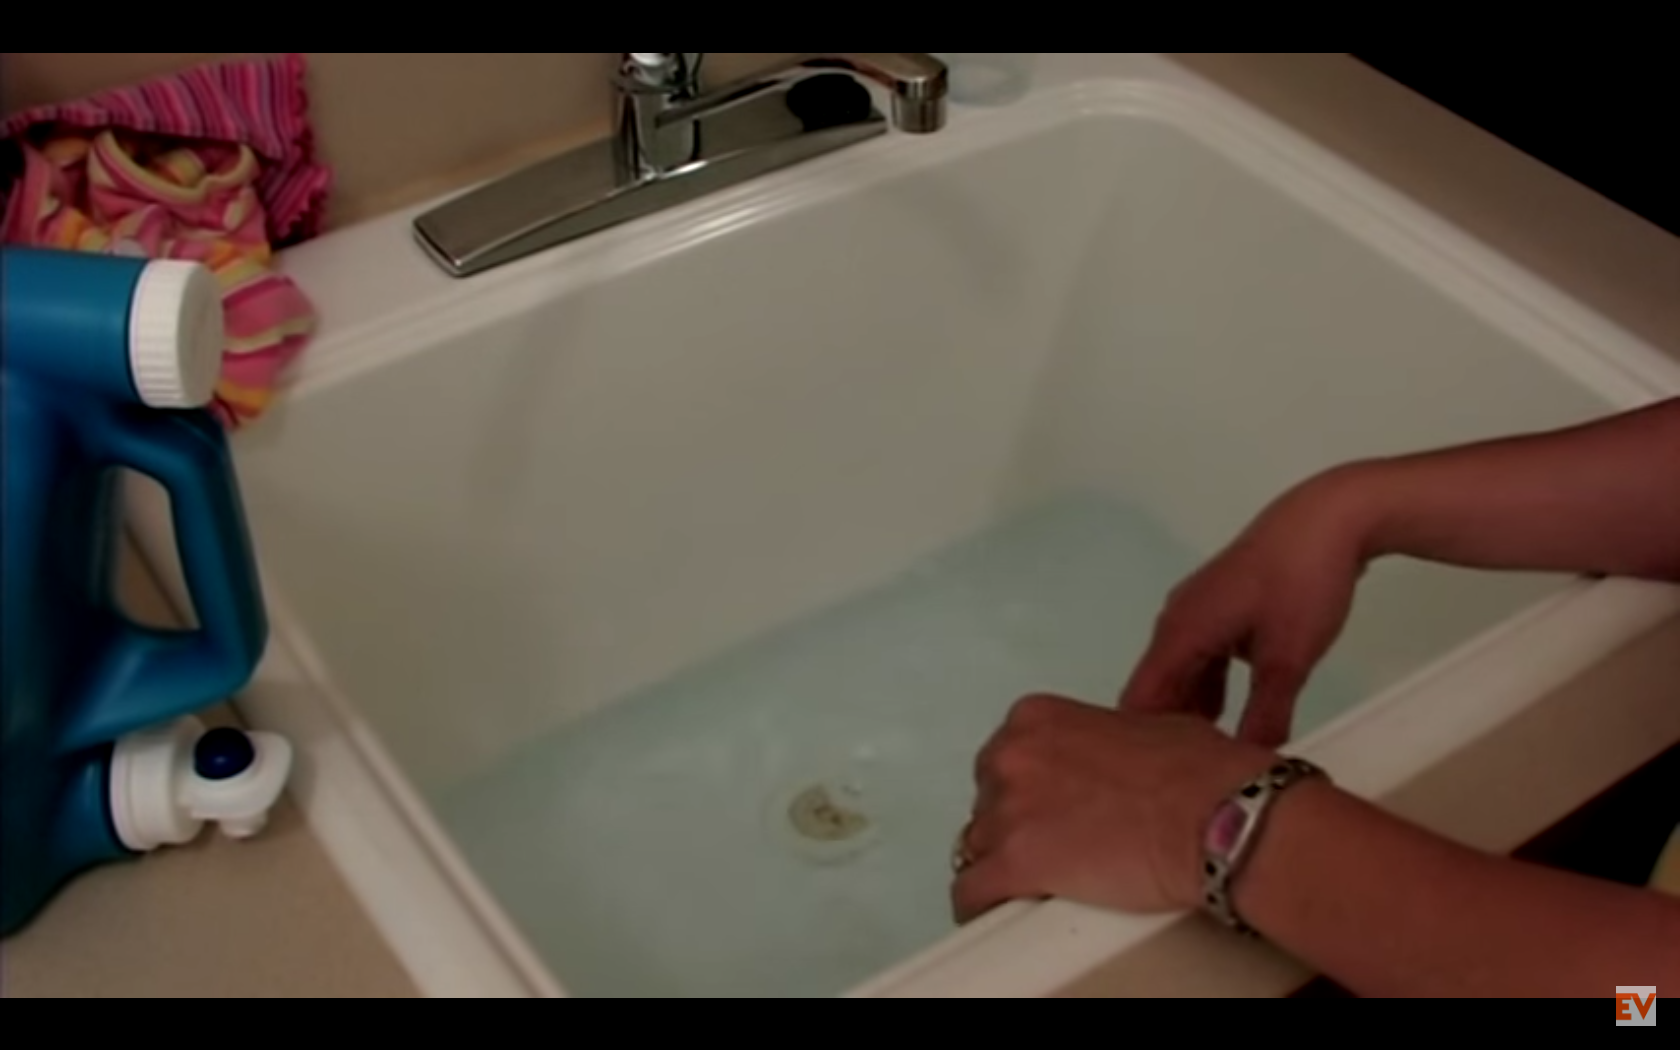
\includegraphics[width=0.95\linewidth]{img/results/activity_classification/results_visualization_classification_10}
\end{subfigure}

\begin{subfigure}[b]{.4\textwidth}
  \texttt{}
\end{subfigure}%
\begin{subfigure}[b]{.6\textwidth}
  \centering
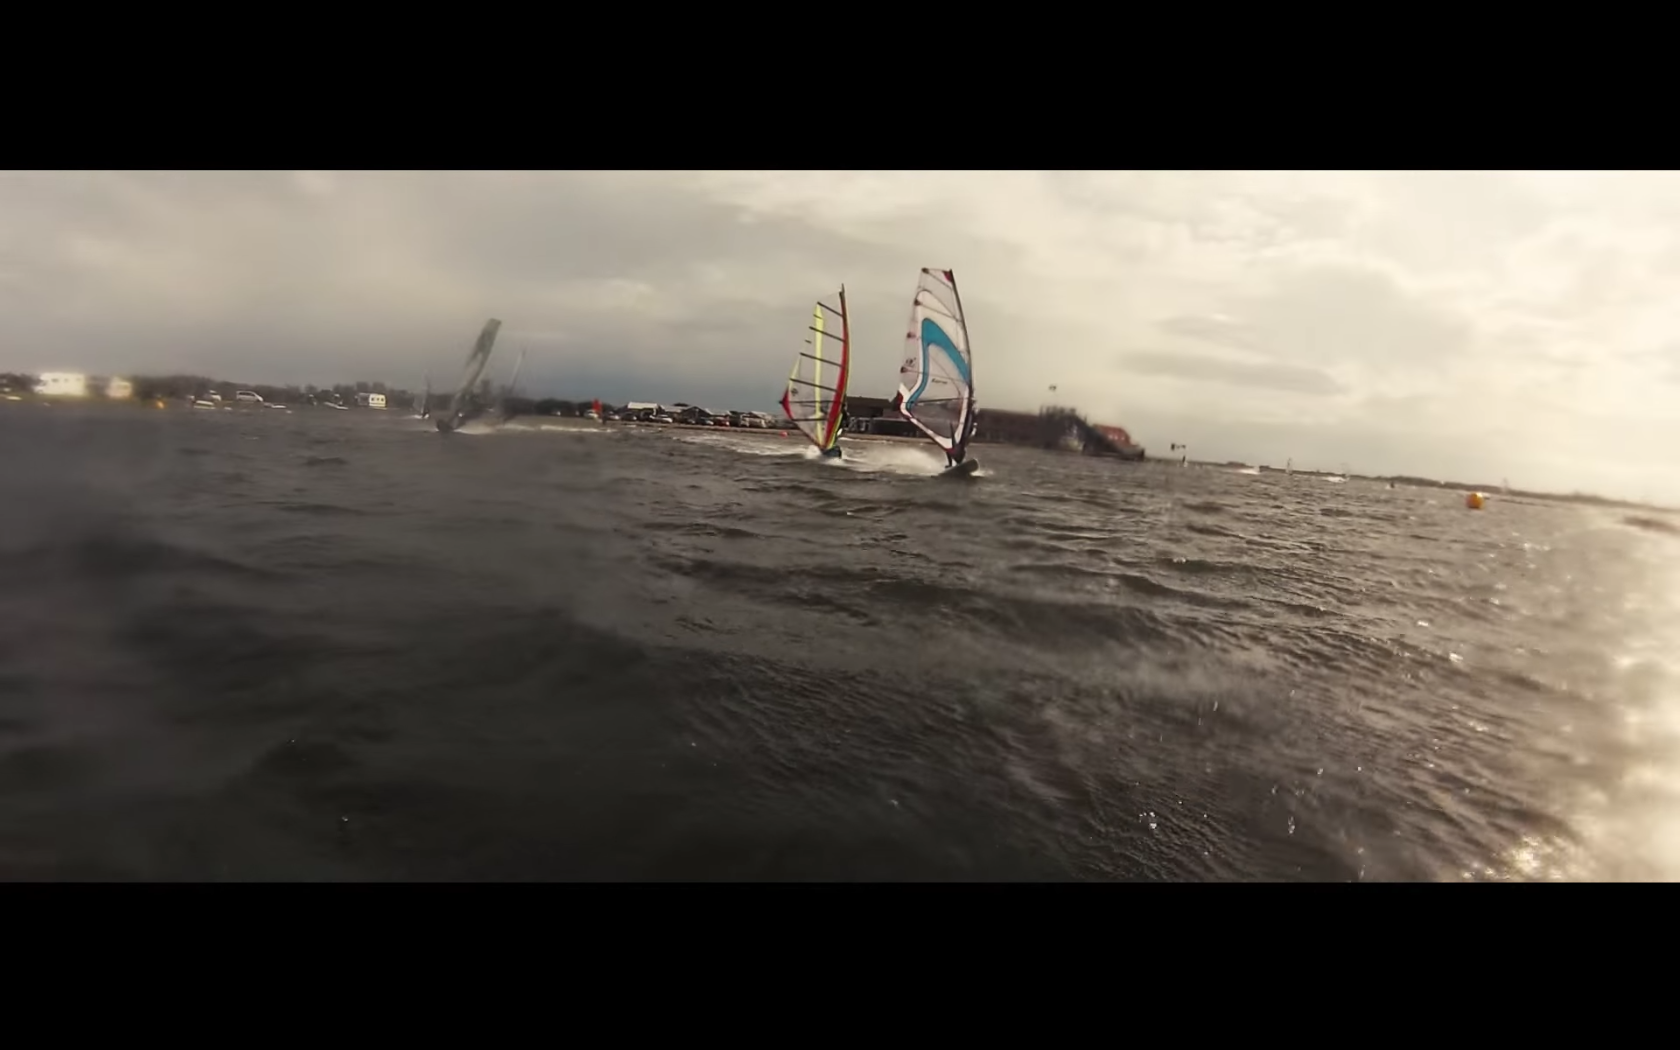
\includegraphics[width=0.95\linewidth]{img/results/activity_classification/results_visualization_classification_11}
\end{subfigure}

\begin{subfigure}[b]{.4\textwidth}
  \texttt{}
\end{subfigure}%
\begin{subfigure}[b]{.6\textwidth}
  \centering
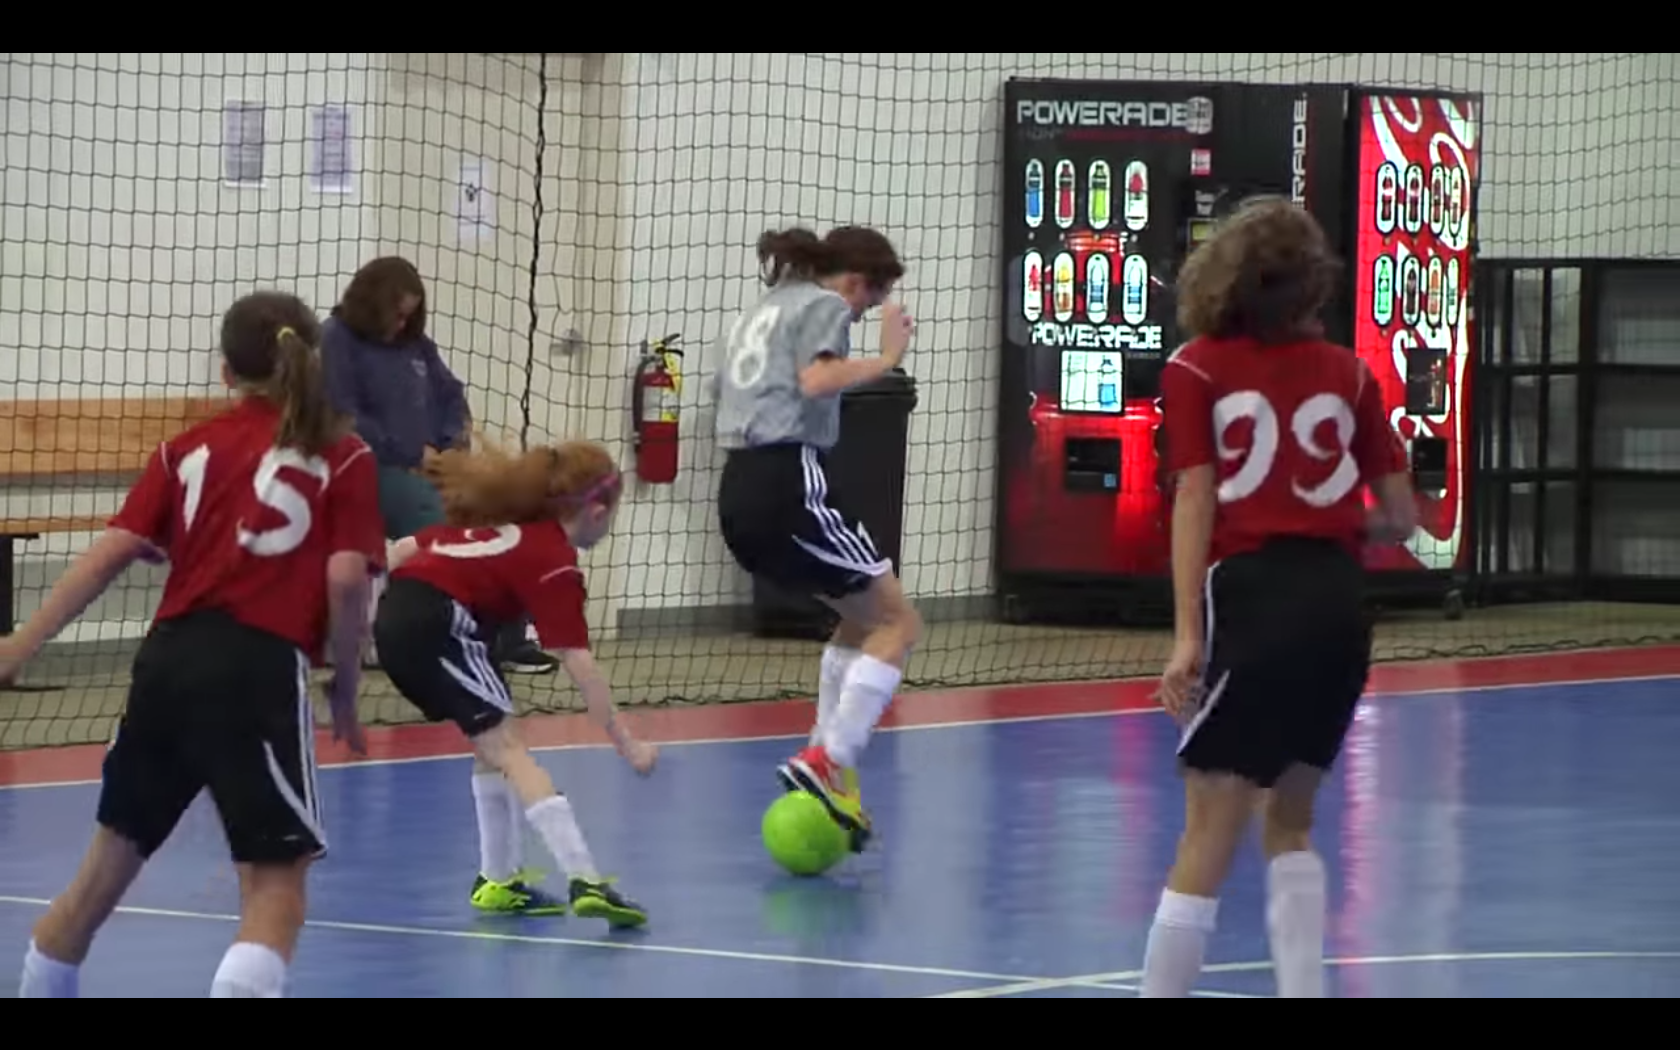
\includegraphics[width=0.95\linewidth]{img/results/activity_classification/results_visualization_classification_12}
\end{subfigure}

\caption{Results for the classification task}
\label{fig:results_visualization_classification_annex_2}
\end{figure}


\begin{figure}[H]
\begin{center}
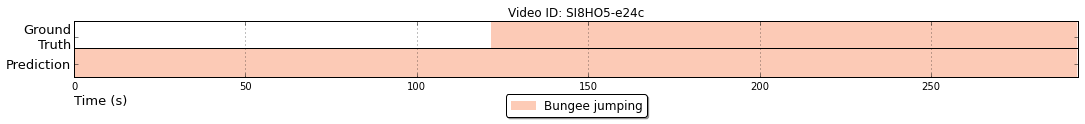
\includegraphics[width=1\linewidth]{img/results/activity_detection/activity_temporal_localization_12}
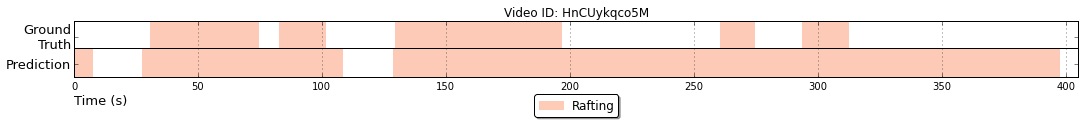
\includegraphics[width=1\linewidth]{img/results/activity_detection/activity_temporal_localization_13}
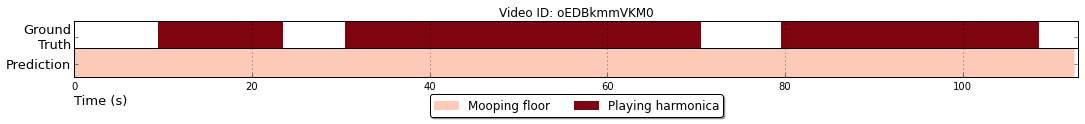
\includegraphics[width=1\linewidth]{img/results/activity_detection/activity_temporal_localization_14}
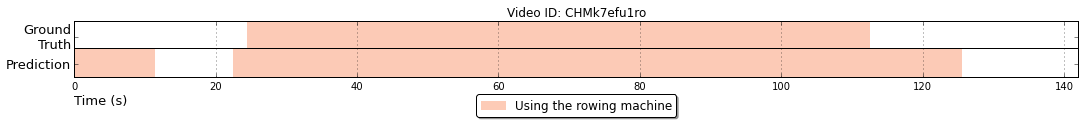
\includegraphics[width=1\linewidth]{img/results/activity_detection/activity_temporal_localization_15}
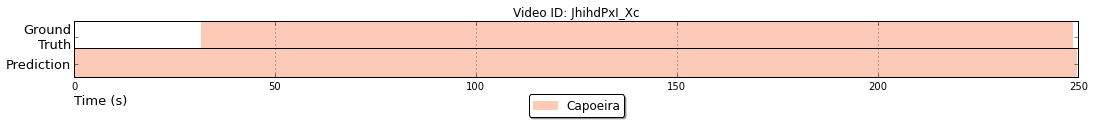
\includegraphics[width=1\linewidth]{img/results/activity_detection/activity_temporal_localization_16}
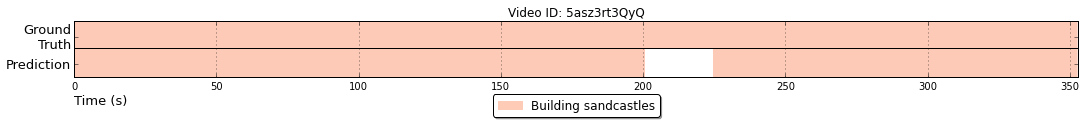
\includegraphics[width=1\linewidth]{img/results/activity_detection/activity_temporal_localization_17}
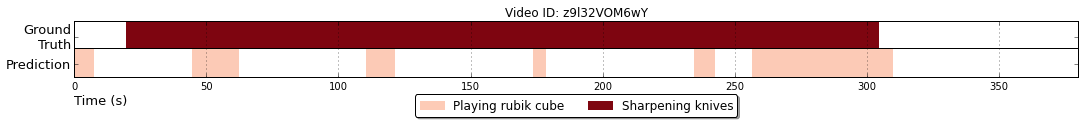
\includegraphics[width=1\linewidth]{img/results/activity_detection/activity_temporal_localization_18}
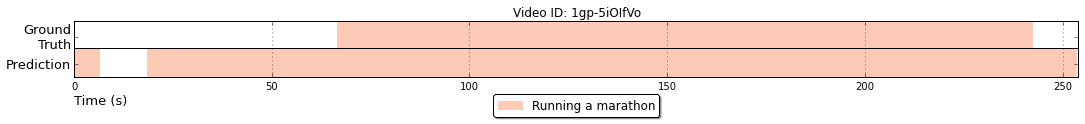
\includegraphics[width=1\linewidth]{img/results/activity_detection/activity_temporal_localization_19}
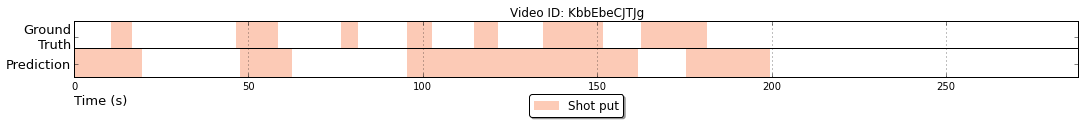
\includegraphics[width=1\linewidth]{img/results/activity_detection/activity_temporal_localization_20}
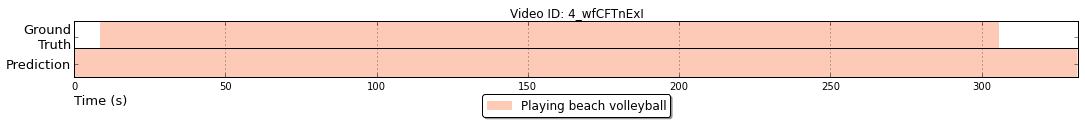
\includegraphics[width=1\linewidth]{img/results/activity_detection/activity_temporal_localization_21}
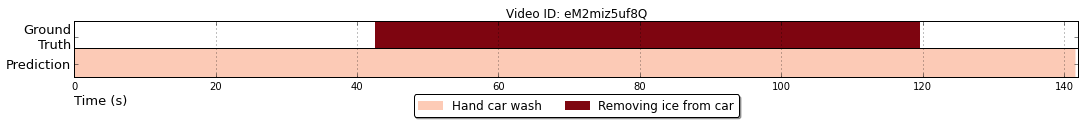
\includegraphics[width=1\linewidth]{img/results/activity_detection/activity_temporal_localization_22}
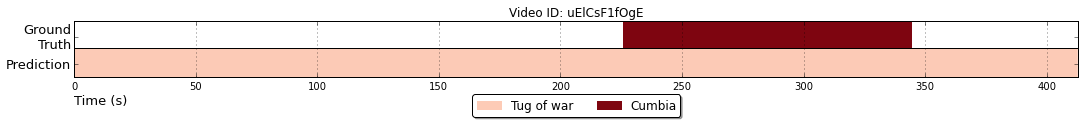
\includegraphics[width=1\linewidth]{img/results/activity_detection/activity_temporal_localization_23}
\end{center}
\caption{Temporal activity localization prediction done by the proposed neural network.}
\label{fig:results_visualization_detection_annex_1}
\end{figure}

\begin{figure}[H]
\begin{center}
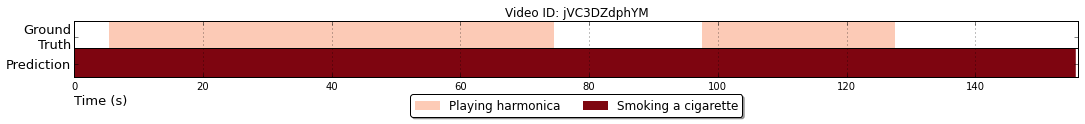
\includegraphics[width=1\linewidth]{img/results/activity_detection/activity_temporal_localization_24}
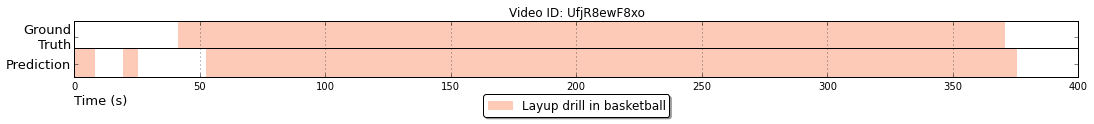
\includegraphics[width=1\linewidth]{img/results/activity_detection/activity_temporal_localization_25}
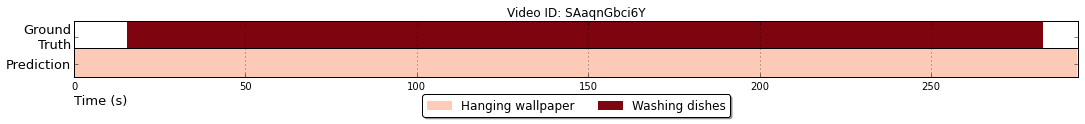
\includegraphics[width=1\linewidth]{img/results/activity_detection/activity_temporal_localization_26}
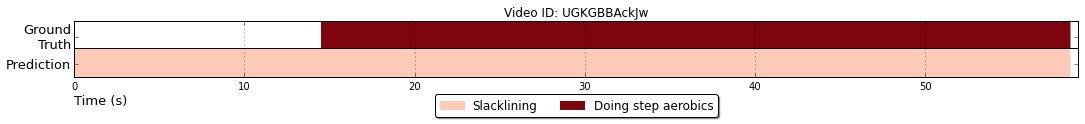
\includegraphics[width=1\linewidth]{img/results/activity_detection/activity_temporal_localization_27}
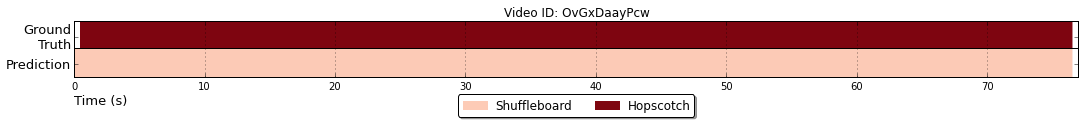
\includegraphics[width=1\linewidth]{img/results/activity_detection/activity_temporal_localization_28}
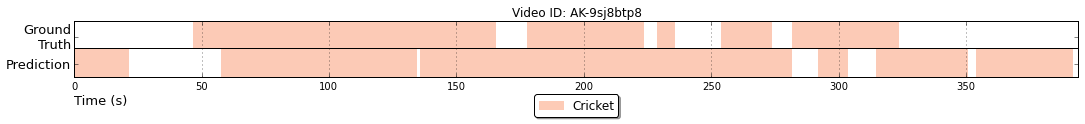
\includegraphics[width=1\linewidth]{img/results/activity_detection/activity_temporal_localization_29}
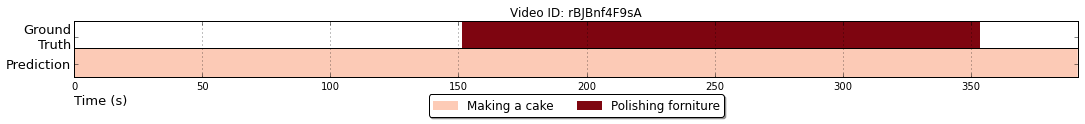
\includegraphics[width=1\linewidth]{img/results/activity_detection/activity_temporal_localization_30}
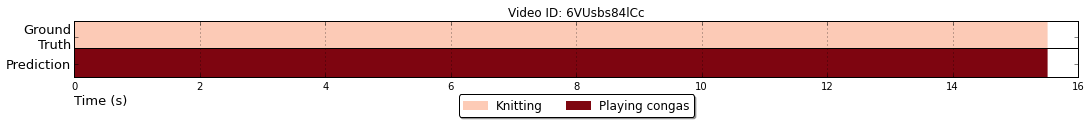
\includegraphics[width=1\linewidth]{img/results/activity_detection/activity_temporal_localization_31}
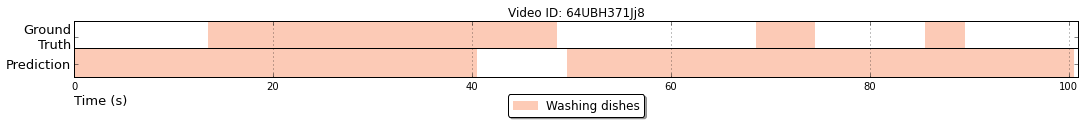
\includegraphics[width=1\linewidth]{img/results/activity_detection/activity_temporal_localization_32}
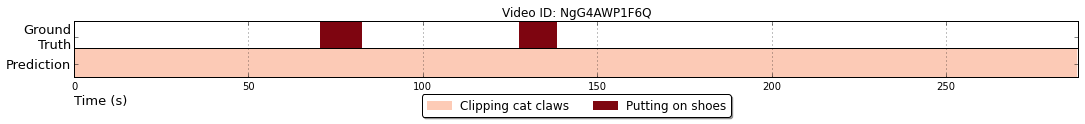
\includegraphics[width=1\linewidth]{img/results/activity_detection/activity_temporal_localization_33}
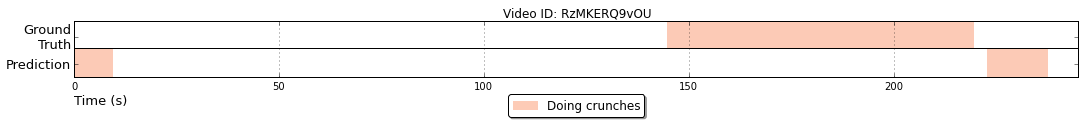
\includegraphics[width=1\linewidth]{img/results/activity_detection/activity_temporal_localization_34}
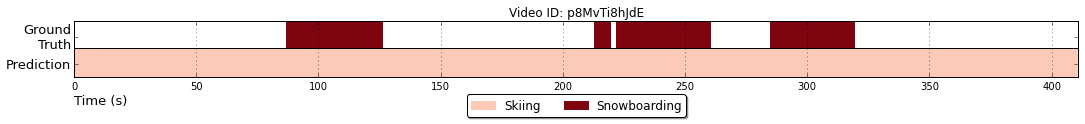
\includegraphics[width=1\linewidth]{img/results/activity_detection/activity_temporal_localization_35}
\end{center}
\caption{Temporal activity localization prediction done by the proposed neural network.}
\label{fig:results_visualization_detection_annex_2}
\end{figure}

\chapter{Notebook Paper}

At the appendix there is the notebook submitted to the ActivityNet Challenge 2016 explaining the work done for to face the challenge.
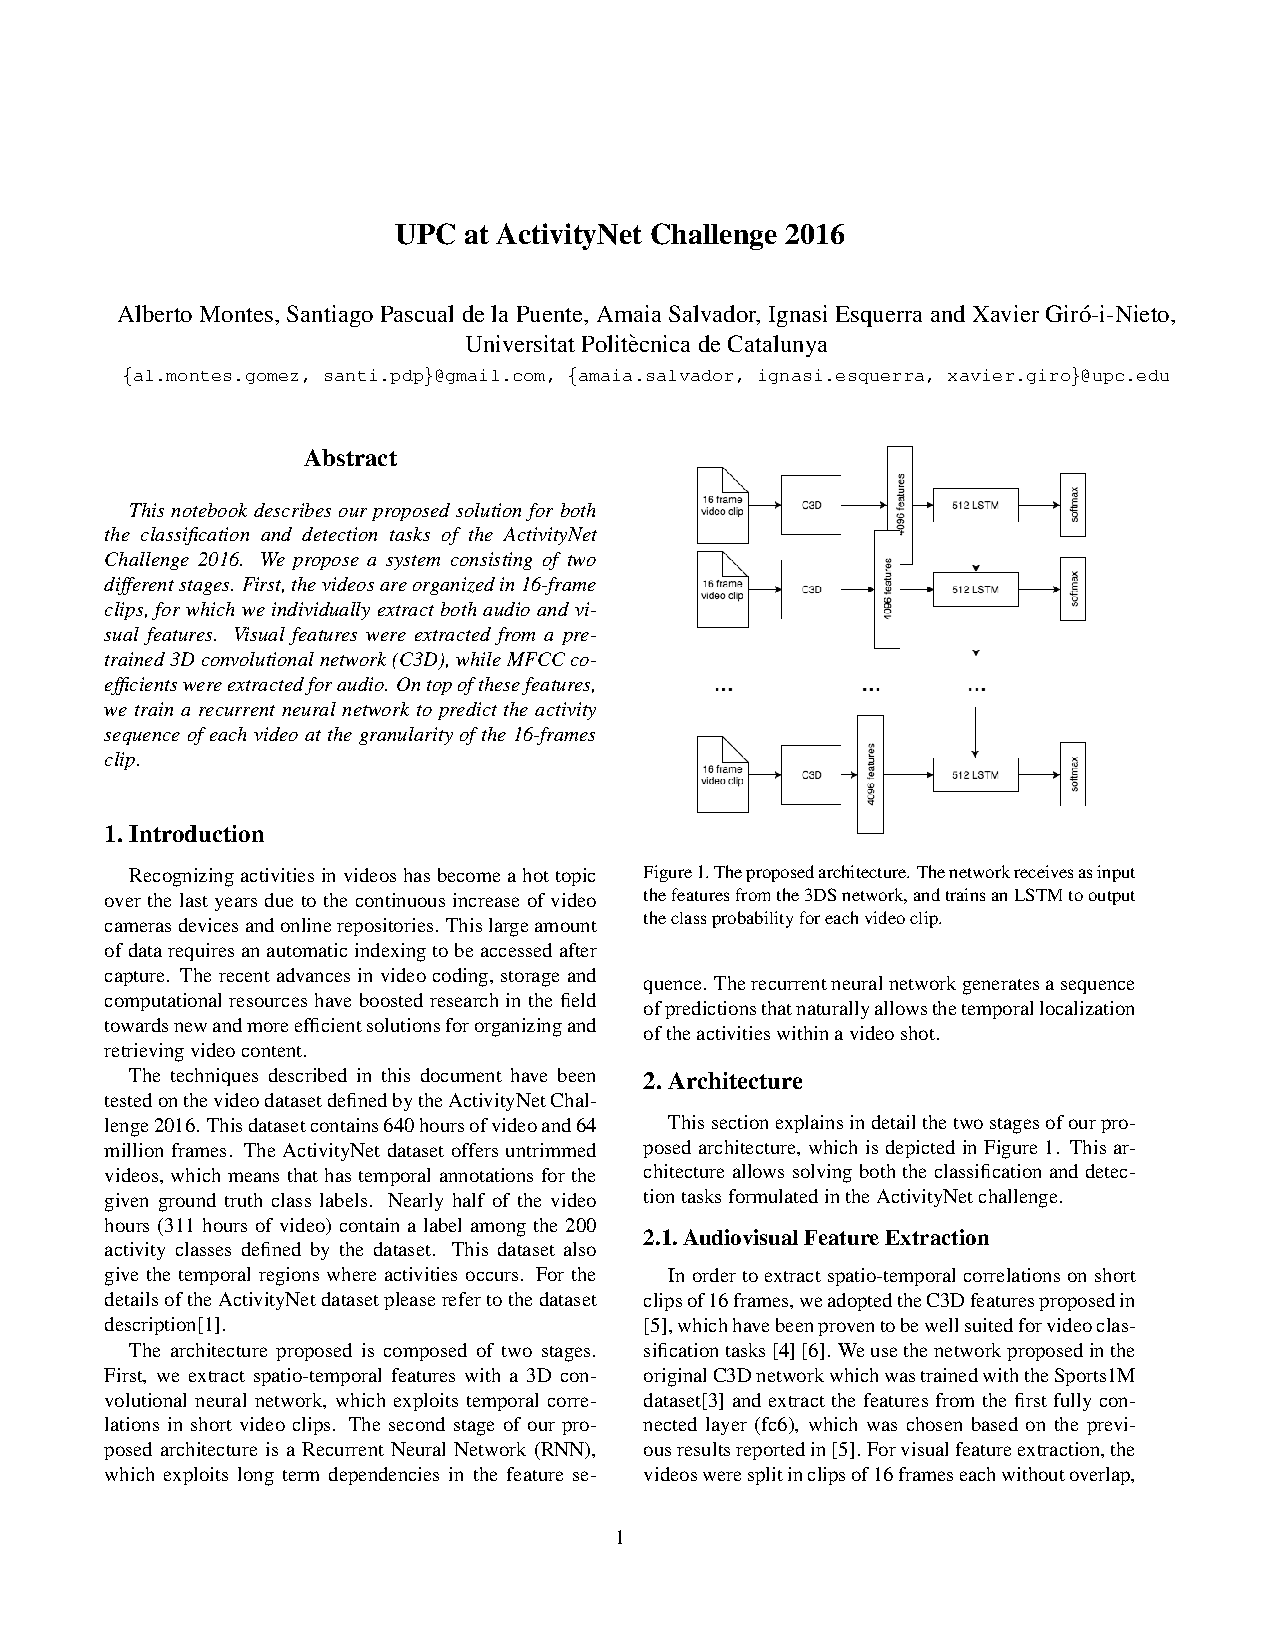
\includepdf[pages={-}]{annex/upc_activitynet_challenge.pdf}



\bibliographystyle{plain}
%%\bibliography{refs}


\end{document}
